\documentclass[12pt,a4paper]{article}
\usepackage[UTF8]{ctex}
\usepackage{amsmath,amssymb}
\usepackage{xcolor}
\usepackage{hyperref}
\usepackage{geometry}
\usepackage{graphicx}
\geometry{margin=2.5cm}

\title{GPU Demo / GPU 演示}
\author{QuoNic}
\date{}

\begin{document}
\maketitle

\begin{center}
\textbf{Tools / 工具} | 难度：初级 | 预计时间：5 分钟
\end{center}

\tableofcontents
\newpage

\section{为什么需要？}

GPU 加速可以显著提高量子模拟的速度。

\subsection{经典局限}
\begin{itemize}
  \item CPU 模拟量子电路慢
  \item 对于大规模电路，CPU 效率低
\end{itemize}

\subsection{量子优势}
\begin{itemize}
  \item GPU 可以并行处理大量量子态
  \item 显著提高模拟速度
  \item 适用于大规模量子电路
\end{itemize}

\subsection{实际应用}
\begin{itemize}
  \item 量子模拟
  \item 量子算法开发
  \item 量子硬件测试
\end{itemize}

\section{快速上手}

\begin{verbatim}
from quonic import qgate, qshow
from quonic.gates import H

# GPU 加速
qgate(H, 0)
qshow(backend='gpu')
\end{verbatim}

\textbf{预期输出}：
\begin{verbatim}
backend: gpu | shots: 1024
Result:
  |0>     512  ( 50.0%)
  |1>     512  ( 50.0%)
\end{verbatim}

\section{原理详解}

\subsection{电路图}

\begin{center}
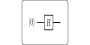
\includegraphics[width=0.6\textwidth]{../../images/gpu_demo_circuit.svg}
\end{center}

\subsection{数学推导}

GPU 加速：
\begin{equation}
\text{Speedup} = \frac{T_{\text{CPU}}}{T_{\text{GPU}}}
\end{equation}

\subsection{几何解释}

GPU 可以并行处理大量量子态。每个 GPU 核心可以处理一个量子态分量。

\section{代码详解}

\begin{verbatim}
from quonic import qgate, qshow
from quonic.gates import H

# GPU 后端
qgate(H, 0)
qshow(backend='gpu')

# CPU 后端（对比）
qshow(backend='native')
\end{verbatim}

\section{进阶用法}

\subsection{场景 1：大规模电路}

\begin{verbatim}
from quonic import qgate, qshow
from quonic.gates import H, CX

# 大规模电路
for i in range(20):
    qgate(H, i)
for i in range(19):
    qgate(CX, i, i+1)
qshow(backend='gpu')
\end{verbatim}

\section{适用场景}

\subsection{量子模拟}

GPU 加速可以显著提高量子模拟的速度。对于大规模量子电路，GPU 比 CPU 快得多。

\subsection{量子算法开发}

GPU 加速可以加快量子算法的开发和测试。

\section{常见问题}

\subsection{GPU 加速需要什么硬件？}

GPU 加速需要 NVIDIA GPU 和 CUDA 支持。

\subsection{GPU 加速的性能如何？}

GPU 加速的性能取决于 GPU 型号和电路规模。对于大规模电路，GPU 可以比 CPU 快 10-100 倍。

\section{学习路径}

\subsection{前置知识}
\begin{itemize}
  \item 量子模拟
  \item GPU 编程
  \item CUDA
\end{itemize}

\subsection{继续学习}
\begin{itemize}
  \item 量子硬件
  \item 量子编译
  \item 量子优化
\end{itemize}

\section{完整示例代码}

\subsection{示例 1：基本 GPU 演示}

\begin{verbatim}
from quonic import qgate, qshow
from quonic.gates import H

qgate(H, 0)
qshow(backend='gpu')
\end{verbatim}

\section{下载}

\begin{itemize}
  \item [gpu\_demo.py](https://github.com/ChrisLee0721/QuoNic/blob/main/examples/gpu_demo/gpu_demo.py)
\end{itemize}

\end{document}
